\documentclass[conference]{IEEEtran}
\IEEEoverridecommandlockouts
% The preceding line is only needed to identify funding in the first footnote. If that is unneeded, please comment it out.
\usepackage{cite}
\usepackage{amsmath,amssymb,amsfonts}
%\usepackage{algorithmic}
\usepackage{graphicx}
\usepackage{textcomp}
\usepackage{xcolor}
\def\BibTeX{{\rm B\kern-.05em{\sc i\kern-.025em b}\kern-.08em
    T\kern-.1667em\lower.7ex\hbox{E}\kern-.125emX}}
\begin{document}

\title{Attentional Trees And Robotics: Towards an Optimal Executive Framework Meeting High-level Decision Making and Control Layer Features.\\
}

\author{\IEEEauthorblockN{1\textsuperscript{st} Pilar de la Cruz}
\IEEEauthorblockA{\textit{Intelligent And Interactive Systems Department} \\
\textit{University of Innsbruck}\\
Innsbruck, Austria \\
pilar.de-la-cruz@uibk.ac.at}
\and
\IEEEauthorblockN{2\textsuperscript{nd} Matteo Saveriano}
\IEEEauthorblockA{\textit{Intelligent And Interactive Systems Department} \\
\textit{University of Innsbruck}\\
Innsbruck, Austria \\
matteo.saveriano@uibk.ac.at}
}

\maketitle

\begin{abstract}
(Brainstorm) Motivation: HRI. Attentional robot - flexible, if possible event-based. Introduce behavior tree trend. Potential in robotics, yet too high level. Merge. JSON. What is this system providing as new? Why is it convincing?
\end{abstract}

\begin{IEEEkeywords}
behavior trees, robotics, event-based, json
\end{IEEEkeywords}

\section{Introduction}
\subsection{Behavior Trees (Brainstorm)}
\begin{itemize}
\item Ticking - the ability to tick allows for work between executions without multi-threading
\item Priority Handling - switching mechansims that allow higher priority interruptions is very natural
\item Simplicity - very few core components, making it easy for designers to work with it
\item Dynamic - change the graph on the fly, between ticks or from parent behaviours themselves
\end{itemize}
\subsection{Behavior Trees Limitations (Brainstorm)}
\subsection{How Limitations can be overcome: JSON (Brainstorm)}
JSON is a standard format for data exchange inspired by JavaScript. Generally, JSON is in string or text format.
This schema provides (1) simplicity due to its compact description of information, (2) flexibility due to its abstract base representation of tasks and (3) modularity due to the definition of subtrees which can be added and/orremoved on the fly in whatever position of Behavior Tree.
\subsection{What is this document about (Brainstorm)}
\subsection{Describe Sections Structure and Content}
\section{Related Works}
Add Matteo's system. Add SoA Behavior Trees.


\section{System Overview}
Attentional Trees framework aims at integrating the following features:
\begin{enumerate}
\item JSON schema conversion into Behavior Trees 
\item Task planner based on Behavior Trees
\item Priority handling of tasks based on the emphasis value \cite{b2}
\item Event-based approach of Behavior Tree  execution
\end{enumerate}
\subsubsection*{JSON Parsing}
 A typical JSON schema consists of a list of string objects. The first object element defines the root of the Behavior Tree. The remaining object elements are defined as subtrees and will be added recursively as children from the root. Each object contains properties \verb|name|, \verb|type|, \verb|father|, \verb|children| and \verb|parameters|, which provide with information about the Behavior Tree node types as well as additional attributes for pre-and post-conditioning handling, priority execution and any additional information. 
 
 \begin{verbatim}
{
    "name":"selector01",
    "type":"selector",
    "father": "sequence01",
    "children": ["isReached","reach"],
    "parameters": [["emphasis", 1]]
}


\end{verbatim}
\subsection{Task Planning}
\subsection{Priority Handling}
\subsection{Event-Based Behavior Tree}

\section*{Implementation}
The framework platform of Attentional Trees is based on the open-source py$\_$trees\cite{b4} library. py$\_$trees is compatible with ROS and provides the easiness and quickness of an implementation based in python language. Moreover, decoding operations becomes specially intuitive thanks to the in-built mapping between container and value (JSON objects to Python objects and viceversa) based on Python standard libraries.
\section*{Simulations}
In order to test the requirements described in section above, the following demo programs have been implemented\footnote{These are available on:}
\begin{itemize}
\item \verb|json-tree.py|. This program focuses on (1) loading JSON schema and (2) mapping into a Behavior Tree based on PA-BT approach \cite{b3}.

\begin{figure}
  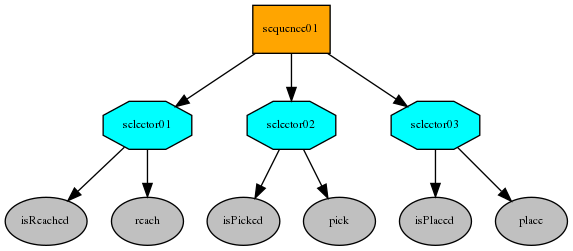
\includegraphics[width=\linewidth]{demo-json.png}
  \caption{Tree expansion rendered from json schema rendered in .dot graph}
  \label{fig:json-tree}
\end{figure}

\item \verb|emphasis-tree.py|. This program focuses on high-priority handling based on access to emphasis value\cite{b1}.
\item \verb|attentional-tree.py|. This program focuses on event-based task execution of Behavior Trees. Tick signals are not periodically sent, but triggered by special events handled in the control layer.
\end{itemize}
\section*{Discussion}




\begin{thebibliography}{00}
\bibitem{b1} Add Matteo's paper and page of emphasis description
\bibitem{b2}https://www.guru99.com/python-json.html
\bibitem{b3} Behavior Tree book
\bibitem{b4} https://py-trees.readthedocs.io/en/devel/
\end{thebibliography}


\end{document}
